% !TeX document-id = {adfd8c77-9aa9-43e7-acaa-af378587f0c7}
% !TeX TXS-program:compile = txs:///pdflatex/[--shell-escape]
\documentclass{article}

\usepackage[utf8]{inputenc}
\usepackage[T1]{fontenc}
\usepackage{color}
\usepackage{soul}
\usepackage{amsmath}
\usepackage{amssymb}
\usepackage{listings}
\usepackage{minted}
\usepackage{hyperref}
\usepackage{graphicx}
\usepackage{calc}
\usepackage{enumitem}
\usepackage{standalone}

\usepackage{tikz}
\usetikzlibrary{datavisualization}
\usetikzlibrary{datavisualization.formats.functions}

\graphicspath{{img/}}
\setlength{\parindent}{0pt}

\begin{document}

\title{CW 19 summary}
\author{Alexander Pastor}
\date{08.05.2017}
\maketitle
\tableofcontents
\newpage

\section{Understanding RF Specifications}

\subsection{Basic Terminology}

\emph{digitizer amplitude error}

The following formula provides the dampening or attenuation factor E of the digitizer:

\begin{equation}
	E = 1- \frac{R}{\sqrt{1+R^2}}
\end{equation}

\medskip

A X-Hz digitizer is defined to have $ E = \frac{1}{\sqrt{2}}$ at the frequency X, which implies $R=1$ for the frequency X. X is called bandwidth of the digitizer in this context, and R is the ratio of the digitizer bandwidth and the maximum frequency of interest $\frac{f_d}{f_i}$.

\begin{figure}[h]
	\centering
	\label{amplitude_error}
	\documentclass[border=2mm,tikz]{standalone}
\usepackage{tikz}
\usetikzlibrary{datavisualization}
\usetikzlibrary{datavisualization.formats.functions}
\begin{document}
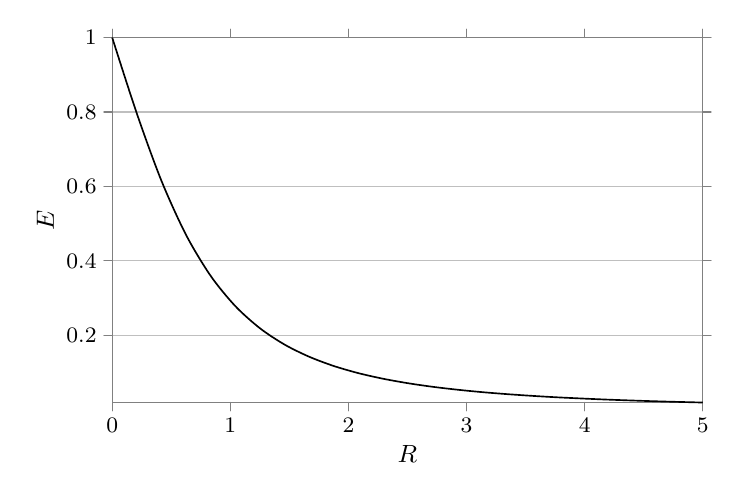
\begin{tikzpicture}
\datavisualization [scientific axes,
					y axis=grid,
                    y axis={label={$E$}},
                    x axis={label={$R$}},
                    visualize as smooth line,
                    scale = 1.5
                   ]

data [format=function]
{
  var x : interval [0:5];
  func y = 1 - ((\value x)/(sqrt(1 + \value x * \value x)));
};
\end{tikzpicture}
\end{document}
	\caption{Digitization error verus bandwidth ratio}
\end{figure}

It is recommended by NI to have X be 3 to 5 times higher than the frequency of interest. This corresponds to errors or dampening between 1.94\% and 5.13\% 

\bigskip

\emph{rise time}

Rise time is defined as the time a signal needs to rise from 10\% to 90\% of its steady-state or periodic maximum.

\bigskip

\begin{itemize}
	\item The rise time of a simple RC-circuit is about $\frac{0.35}{RC}$.
	\item The formula to calculate the total rise time of a digitized signal is: $$ T_{r_t} = \sqrt{{T_{r_s}}^2 + {T_{r_d}}^2}$$
	\item In order to minimize rise time errors NI recommends to have $T_{r_d}$ be around $\frac{1}{3}$ and $\frac{1}{5}$ of $T_{r_s}$.
\end{itemize}

\emph{Nyquist Theorem}

The bandwidth of the digitizer must be at least 2 times the maximum frequency of the signal to avoid aliasing. 

\medskip

$\Leftrightarrow$ To extinguish aliasing in the passband one either has to make sure the Nyquist Theorem is matched or apply a lowpass filter to limit the signal's bandwidth.

\bigskip

\emph{phase noise}

\bigskip

\emph{resolution bandwidth}

\bigskip

\emph{noise density}

\bigskip

\emph{dynamic range}

\bigskip

\emph{voltage standing wave ratio (VSWR)}

\bigskip

\emph{frequency response}

\bigskip
 
\emph{modulation error ratio (MER)}

\bigskip

\emph{error vector magnitude (EVM)}

\bigskip

\emph{third-order intercept (TOI)}

\section{Physical Layer Challenge}

\subsection{Basic Terminology}

\subsubsection{FIR Filters}

\emph{passband, transitionband, stopband}

The passband is the frequency band that is not attenuated band of a filter, i.e. that band of allowed frequencies. The stopband is the band that a filter stops, or attenuates strong enough, so that the signal amplitude for those frequencies is below the stopband threshold. The transitionband is an attenuated band between passband and stopband.  

\bigskip

\emph{filter tap}

A filter tap is a (coefficient, delay) pair. The number of taps is often denoted as N. This number is a good mesaure for the amount of filtering, the required space and the amount of calculation required by the filter. 

\subsubsection{Frame Synchronization}

\emph{frame preamble}

\bigskip

\emph{CRC-based framing}

\bigskip

\emph{self-clocking signal}

\bigskip

\emph{bit slip}

A lost bit or an extra bit.

\subsection{FIR Filters vs. IIR Filters} 

\subsection{iNets PHY Layer}

\section{GNU Radio Techniques}

\subsection{Creating a hierarchical block directly in GRC}

\subsection{Read and Write Stream Tags}

\section{Good to Know...}

\subsection{Python}

\subsection{\LaTeX}

I learned...

\begin{itemize}
	\item ... when to use \href{https://tex.stackexchange.com/questions/246/when-should-i-use-input-vs-include}{input or include}
	\item ... some tikz basics
\end{itemize}

\end{document}